\documentclass[11pt,a4paper]{article}

% ── Packages ──
\usepackage[margin=2.5cm]{geometry}
\usepackage{amsmath,amssymb}
\usepackage{booktabs}
\usepackage{longtable}
\usepackage{xcolor}
\usepackage{hyperref}
\usepackage{enumitem}
\usepackage{tikz}
\usepackage{fontspec}
\setmainfont{Liberation Serif}

\hypersetup{
  colorlinks=true,
  linkcolor=blue!60!black,
  urlcolor=blue!60!black
}

\definecolor{headcolor}{HTML}{1B365D}
\definecolor{subcolor}{HTML}{7A9CC6}

\begin{document}

% ── Title ──
\begin{center}
{\LARGE\bfseries\color{headcolor} Research Methodology \& Experimental Design}\\[0.5cm]
{\large Institutional Common Ownership and Executive Mobility}\\[0.3cm]
{\normalsize Kun Zhang \quad·\quad University of Navarra}\\[0.2cm]
{\normalsize Advisor: Jos\'{e} Azar}
\end{center}
\vspace{-0.3cm}
\rule{\textwidth}{0.4pt}

% ── Contents ──
\tableofcontents
\newpage

% ═══════════════════════════════════════════════
\section{Research Question}
% ═══════════════════════════════════════════════

This study investigates the causal effect of institutional common ownership on C-suite executive mobility. The central research question is:

\begin{quote}
{\bf Does institutional common ownership suppress or facilitate the movement of C-suite executives across connected firms?}
\end{quote}

We exploit the exogenous shock of BlackRock's acquisition of Barclays Global Investors (BGI), completed in December 2009, to identify how changes in common ownership network structure affect executive mobility patterns. The theoretical framework involves two competing hypotheses:

\begin{enumerate}[leftmargin=*]
  \item {\bf Shadow Non-Compete:} Common owners coordinate to suppress labor market competition across their portfolio firms, reducing executive mobility (Ant\'{o}n et al., 2018)
  \item {\bf Internal Labor Market (ILM):} Common ownership networks build bridges between firms, facilitating directed executive movement (Tate \& Yang, 2015)
\end{enumerate}

{\color{red}\bf Empirical conclusion: The data reject the Shadow NCA hypothesis and support the ILM channel.}

\newpage

% ═══════════════════════════════════════════════
\section{Data Sources}
% ═══════════════════════════════════════════════

\subsection{Core Databases}

\begin{longtable}{p{3.5cm}p{3cm}p{3cm}p{3cm}}
\toprule
\textbf{Database} & \textbf{Content} & \textbf{Time Span} & \textbf{Size} \\
\midrule
Thomson Reuters 13F & Institutional quarterly holdings & 2007--2008, 2010--2011 & 58,929,118 rows \\
Compustat & Firm financials & 2005--2015 & — \\
ExecuComp & Executive compensation \& mobility & 2005--2015 & 244,857 obs (cleaned) \\
CRSP Stock & Stock prices \& returns & 2005--2015 & — \\
CRSP Names & Firm names \& identifiers & — & — \\
Orbis (BvD) & Director appointments \& moves & 2000--2025 & 14,220 firms, 1,417,530 person-role records \\
\bottomrule
\end{longtable}

\subsection{13F Data Limitation}\label{sec:13f_limit}

An unavoidable constraint: due to data acquisition windows, we have only {\bf two time cross-sections} of institutional holdings — pre-merger (2007--2008) and post-merger (2010--2011). Consequently, \(\lambda_{jk}\) can only be computed once for each period (\(\lambda_{jk}^{\text{Pre}}\) and \(\lambda_{jk}^{\text{Post}}\)), yielding no annual panel of \(\lambda\).

This limitation, however, does {\bf not} preclude the core Event Study logic (see Section~\ref{sec:eventstudy}).

\subsection{Sample Scale}

\begin{table}[h!]
\centering
\begin{tabular}{lr}
\toprule
\textbf{Metric} & \textbf{Value} \\
\midrule
13F raw rows & 58,929,118 \\
Matched firms & 2,884 (panel) / 922+1,035 (lambda) \\
Regression sample (executive-years) & 31,959 \\
Firm-pairs & 1,070,174 \\
Pairs with observed moves & 2,516 \\
Orbis director moves (total) & 24,716 \\
Moves with \(\lambda_{jk}\) data & 2,659 \\
Pre-crisis mobility rate (2005--2008) & 6.45\% \\
Post-crisis mobility rate (2010--2014) & 0.53\% \\
\bottomrule
\end{tabular}
\caption{Sample scale summary}
\end{table}

\newpage

% ═══════════════════════════════════════════════
\section{Variable Construction}
% ═══════════════════════════════════════════════

\subsection{Common Ownership Metric \(\lambda_{jk}\)}

We adopt the standard formula from Azar, Schmalz, \& Tecu (2018):

\begin{equation}\label{eq:lambda}
\lambda_{jk} = \frac{\sum_i \beta_{ij} \beta_{ik}}{\sum_i \beta_{ij}^2}
\end{equation}

where \(\beta_{ij}\) is investor \(i\)'s ownership share in firm \(j\). \(\lambda_{jk} \in [0, 1]\) measures the strength of the common ownership link between firms \(j\) and \(k\) through shared institutional investors.

\vspace{0.2cm}

When control rights \(\gamma_{ij}\) differ from cash-flow rights \(\beta_{ij}\), the generalized formula applies:

\begin{equation}
\lambda_{jk} = \frac{\sum_i \gamma_{ij} \beta_{ik}}{\sum_i \gamma_{ij} \beta_{ij}}
\end{equation}

This study uses the standard formula (assuming \(\gamma = \beta\)).

\subsection{Treatment Variable \(\Delta\lambda_{jk}\)}

\begin{enumerate}[leftmargin=*]
  \item Compute \(\lambda_{jk}^{\text{Pre}}\) using pre-merger 13F data (2007--2008)
  \item Compute \(\lambda_{jk}^{\text{Post}}\) using post-merger 13F data (2010--2011)
  \item Treatment variable: \(\Delta\lambda_{jk} = \lambda_{jk}^{\text{Post}} - \lambda_{jk}^{\text{Pre}}\)
\end{enumerate}

Key points:
\begin{itemize}
  \item \(\Delta\lambda_{jk} > 0\): BlackRock-BGI merger strengthened the common ownership link between \(j\) and \(k\)
  \item \(\Delta\lambda_{jk} < 0\): Merger weakened the link (e.g., due to portfolio rebalancing)
  \item Base period benchmark: {\bf 2009 Q3} (the last full quarter before the merger closed)
\end{itemize}

\subsection{Firm-Level Treatment Variable}

As a complementary measure at the firm level, the treatment variable is:

\begin{equation}
\text{BR\_beta\_change}_j = \beta_{j, \text{BlackRock}}^{\text{Post}} - \beta_{j, \text{BlackRock}}^{\text{Pre}}
\end{equation}

i.e., the change in BlackRock's ownership share in firm \(j\). This variable produced robust results in Phases 8--9 (\(+0.0731^{***}\), \(p=0.002\)), but cannot capture inter-firm network relationships.

\newpage

\subsection{Executive Mobility}

\begin{description}[leftmargin=*]
  \item[ExecuComp firm-level:] \(\text{Mobility}_{i,t}\) — whether executive \(i\) changed firms in year \(t\) (0/1), defined as the last employer in year \(t\) differing from the last employer in year \(t-1\)
  \item[ExecuComp directional:] \(\text{Poach}_{i,t}\) — executive moves to a firm held by BlackRock
  \item[Orbis pair-level:] \(\text{Move}_{j,k}\) — a director moved from firm \(j\) to firm \(k\) (extracted chronologically; consecutive appointments of the same person at different firms constitute one directed move)
\end{description}

\subsection{Key Control Variables (ExecuComp firm-level)}

\subsubsection*{Executive Characteristics}
\begin{itemize}[nosep]
  \item Age
  \item Tenure within the firm
  \item Position one year prior to departure (CEO = 1)
\end{itemize}

\subsubsection*{Firm Characteristics}
\begin{itemize}[nosep]
  \item Firm size (\(\log(\text{total assets})\))
  \item Profitability (ROA)
  \item Leverage (total liabilities / total assets)
  \item Book-to-market ratio
  \item R\&D intensity (R\&D / total assets, used for heterogeneity analysis)
\end{itemize}

\subsubsection*{Market-Based Variables (extended)}
\begin{itemize}[nosep]
  \item Log market capitalization (\(\log(\text{mktcap})\))
  \item Annualized stock return
  \item Annualized volatility
\end{itemize}

\subsubsection*{Caveat}
Adding market-based variables reduces the sample from 32K to 14K (56\% missing). The coefficient is stable at \(+0.073\) across all 9 control specifications (all \(p < 0.003\)), but the market-variable subsample yields an insignificant coefficient — a sample selection issue, not a specification issue.

\newpage

% ═══════════════════════════════════════════════
\section{Identification Strategy \& Experimental Design}
% ═══════════════════════════════════════════════

\subsection{Dual-Level Analytical Framework}

This study adopts a {\bf dual-level analysis} strategy to maximize data utilization and address the inherent constraint of 13F data:

\begin{table}[h!]
\centering
\begin{tabular}{p{3cm}p{5cm}p{5cm}}
\toprule
\textbf{Dimension} & \textbf{Firm-Level} & \textbf{Pair-Level} \\
\midrule
Unit of analysis & \((i, t)\) or \((j, t)\) & \((j, k, t)\) \\
Data source & ExecuComp + Compustat & Orbis director records \\
Sample size & 31,959 exec-years & 1,070,174 firm-pairs \\
Treatment variable & BR\_beta\_change & \(\Delta\lambda_{jk}\) \\
Causal framework & Continuous DiD & Pair-level variation \\
\bottomrule
\end{tabular}
\caption{Dual-level analytical framework}
\end{table}

\subsection{Level 1: Firm-Level Continuous DiD}

\begin{equation}\label{eq:firm_did}
\text{Mobility}_{i,t} = \beta_1 (\text{BR\_beta\_change}_j \times \text{Post}_t) + \boldsymbol{\gamma} \mathbf{X}_{i,t} + \eta_j + \eta_t + \varepsilon_{i,t}
\end{equation}

\begin{description}[leftmargin=*]
  \item[Source of identification] Exogenous variation in BR\_beta\_change across firms (differential exposure to the BlackRock-BGI merger shock)
  \item[Post definition] 2010 onward (i.e., the year the merger takes effect)
  \item[Base period] 2009 Q3 (last full quarter before merger completion)
  \item[Clustering] Standard errors clustered at the firm level
\end{description}

\subsubsection*{Long-Difference Specification}

To mitigate the financial crisis dilution effect, we complement with a long-difference specification:

\begin{equation}
\Delta \text{Mobility}_{j} = \beta (\text{BR\_beta\_change}_j) + \boldsymbol{\gamma} \Delta \mathbf{X}_{j} + \varepsilon_{j}
\end{equation}

where \(\Delta \text{Mobility}_j\) is the difference between the 2005--2007 average and the 2012--2014 average.

\newpage

\subsection{Level 2: Pair-Level Analysis}

\subsubsection*{Cross-Sectional Logit / OLS}

\begin{equation}\label{eq:pair_cross}
\text{AnyMove}_{jk} = \beta_1 \Delta\lambda_{jk} + \beta_2 \lambda_{jk}^{\text{Pre}} + \boldsymbol{\gamma} \mathbf{X}_{jk} + \eta_{j,\tau} + \mu_{k,\tau} + \varepsilon_{jk}
\end{equation}

\begin{description}[leftmargin=*]
  \item[AnyMove\(_{jk}\)] (0/1) — whether a director ever moved from \(j\) to \(k\)
  \item[\(\lambda_{jk}^{\text{Pre}}\)] Controls for pre-treatment level effects
  \item[\(\eta_{j,\tau}\)] Origin firm \(\times\) time-period FE
  \item[\(\mu_{k,\tau}\)] Destination firm \(\times\) time-period FE
\end{description}

\subsubsection*{Pair \(\times\) Year Event Study (Equivalent Specification)}\label{sec:eventstudy}

Although \(\Delta\lambda_{jk}\) is constant at the pair level (13F has only two time cross-sections), director moves in Orbis have precise dates. We construct a {\bf pair \(\times\) year panel} and estimate:

\begin{equation}\label{eq:pair_event}
\text{Move}_{jk,t} = \sum_{\tau} \delta_\tau (\Delta\lambda_{jk} \times \mathbf{1}_{\text{year}=\tau}) + \gamma \lambda_{jk}^{\text{Pre}} + \eta_{j,t} + \mu_{k,t} + \varepsilon_{jk,t}
\end{equation}

{\bf Core logic:}

\begin{itemize}
  \item \(\Delta\lambda_{jk}\) is the treatment intensity (time-invariant), not \(\lambda_{jk}\) itself
  \item The Event Study plot shows the marginal explanatory power of the {\em same} \(\Delta\lambda_{jk}\) for \(\text{Move}_{jk,t}\) in {\em different} years
  \item If parallel trends hold: pre-2009 \(\delta_\tau\) should be insignificant (\(\approx 0\))
  \item If the treatment is effective: post-2009 \(\delta_\tau\) should be significantly positive
  \item Fixed effects \(\eta_{j,t}\) and \(\mu_{k,t}\) are absorbed via the FWL theorem prior to OLS to handle the high-dimensional problem
\end{itemize}

\subsection{Fixed Effects Strategy}

\begin{table}[h!]
\centering
\begin{tabular}{p{2.5cm}p{5cm}p{5cm}}
\toprule
\textbf{Specification} & \textbf{Firm-Level} & \textbf{Pair-Level} \\
\midrule
Core FE & Firm FE + Year FE & Origin \(\times\) Year FE + Dest \(\times\) Year FE \\
Robust FE & Exec FE + Firm FE & — \\
Clustering & Firm level & Two-way (origin + dest) \\
FWL absorption & — & High-dim FE absorbed via residualization before OLS \\
\bottomrule
\end{tabular}
\caption{Fixed effect specifications}
\end{table}

\newpage

% ═══════════════════════════════════════════════
\section{Empirical Results}
% ═══════════════════════════════════════════════

\subsection{Firm-Level Core DiD Results}

\begin{table}[h!]
\centering
\begin{tabular}{lcccc}
\toprule
 & \textbf{(1) OLS} & \textbf{(2) +Exec FE} & \textbf{(3) +Firm FE} & \textbf{(4) Long-diff+FE} \\
\midrule
BR\(\Delta\) \(\times\) Post & \(+0.0717^{***}\) & \(+0.0727^{***}\) & \(+0.0731^{***}\) & \(+0.096^{***}\) \\
 & (0.0025) & (0.0022) & (0.0020) & (0.005) \\
R\(^2\) & 0.022 & 0.023 & 0.024 & 0.055 \\
\(N\) & 31,959 & 31,959 & 31,959 & 18,108 \\
\midrule
\multicolumn{5}{l}{\footnotesize \(^{*}p<0.10\), \(^{**}p<0.05\), \(^{***}p<0.01\). SE clustered at the firm level.} \\
\bottomrule
\end{tabular}
\caption{Firm-Level Core DiD Results}
\end{table}

\subsection{Economic Significance}

\begin{itemize}
  \item BR\_beta\_change SD = 0.127
  \item 1 SD increase \(\rightarrow\) +0.93 pp in mobility probability (+19.5\% of mean)
  \item Average treatment effect for affected firms: +1.67 pp (+34.9\% of mean)
\end{itemize}

\subsection{Pair-Level Logit Results}

\begin{table}[h!]
\centering
\begin{tabular}{lcc}
\toprule
 & \textbf{Coefficient} & \textbf{\(p\)-value} \\
\midrule
logit \(\lambda_{jk}^{\text{Pre}}\) & \(+1.546\) & \(< 10^{-124}\) \\
logit \(\Delta\lambda_{jk}\) & \(+0.583\) & \(< 10^{-18}\) \\
\midrule
Marginal effect \(\lambda_{jk}^{\text{Pre}}\) & \(+0.0036\) & — \\
Marginal effect \(\Delta\lambda_{jk}\) & \(+0.0014\) & — \\
\midrule
\(N\) (pairs) & 1,070,174 & — \\
Pairs with moves & 2,516 & — \\
\bottomrule
\end{tabular}
\caption{Pair-Level Logit Regression Results}
\end{table}

\subsubsection*{Interpretation}

Both \(\lambda_{jk}^{\text{Pre}}\) and \(\Delta\lambda_{jk}\) are highly significant, indicating that the level {\em and} change in common ownership independently predict executive mobility. Economically, this confirms that the common ownership network exhibits both a cross-sectional association (high-\(\lambda\) firms have always had more moves) and a causal effect (exogenous network structure change \(\Delta\lambda\) further increases mobility).

\newpage

\subsection{Robustness Summary}

\begin{longtable}{p{5cm}lc}
\toprule
\textbf{Test} & \textbf{Result} & \textbf{Status} \\
\midrule
Controls 0 \(\rightarrow\) 9 & Coefficient stable at \(+0.073\), all \(p < 0.003\) & \(\checkmark\) \\
Drop tenure restriction & \(+0.162^{***}\), \(N = 58,255\) & \(\checkmark\) \\
Post cutoff at 2011 & \(+0.065^{***}\) \((p = 0.005)\) & \(\checkmark\) \\
1\% winsorization & \(+0.101^{***}\) \((p = 0.005)\) & \(\checkmark\) \\
Parallel trends test (firm-level) & \(F\)-test \(p = 0.20\) (fail to reject) & \(\checkmark\) \\
Placebo — 2006 fake treatment & Coef = 0.037, \(p = 0.211\) & \(\checkmark\) \\
Alternative \(\lambda\) aggregation (7 methods) & Mean-gap method wins & \(\checkmark\) \\
R\&D heterogeneity & High +0.099, Low +0.093\(^{**}\) \(\rightarrow\) ILM confirmed & \(\checkmark\) \\
Binary treatment (median split) & Coef = +0.0035, \(p = 0.77\) (null) & \(\checkmark\) (continuous confirmed) \\
\bottomrule
\caption{Robustness Summary}
\end{longtable}

\subsection{Financial Crisis Collapse — ILM Channel Evidence}

Unconditional executive mobility rate collapsed from {\bf 6.45\%} (2005--2008) to {\bf 0.53\%} (2010--2014) — a \(-91.8\%\) decline.

\begin{quote}
{\bf Interpretation:} The ILM is a trust network. Under the shock of the financial crisis, even though common ownership links remained structurally present, firms' risk aversion surged dramatically and they ceased using the network for executive allocation. Trust collapsed \(\rightarrow\) network bridges broke.
\end{quote}

\newpage

% ═══════════════════════════════════════════════
\section{Theoretical Narrative Framework}
% ═══════════════════════════════════════════════

\subsection{Narrative Evolution}

\begin{table}[h!]
\centering
\begin{tabular}{p{3cm}p{5cm}p{5cm}}
\toprule
\textbf{Dimension} & \textbf{Original Hypothesis (Rejected)} & \textbf{Current Narrative} \\
\midrule
Mechanism & Shadow NCA: common ownership suppresses competition, reduces mobility & ILM: common ownership builds network, facilitates mobility \\
Theory basis & Ant\'{o}n et al. (2018) & Tate \& Yang (2015) \\
Empirical support & Binary treatment \(p = 0.77\) (null) & Continuous treatment \(+0.073^{***}\) \\
Data contradiction & Placebo 2007--08 significant & Parallel trends pass \\
\bottomrule
\end{tabular}
\caption{Narrative evolution}
\end{table}

\subsection{Revised Narrative Chain}

\[
\boxed{\text{BlackRock acquires BGI}} \;\longrightarrow\; \boxed{\text{Inter-firm common ownership links strengthen}} \;\longrightarrow\; \boxed{\Delta\lambda_{jk} \uparrow} \;\longrightarrow\; \boxed{\text{Connected-firm executive mobility} \uparrow}
\]

\begin{quote}
{\bf The mechanism is network formation, not mere ownership concentration.}
\end{quote}

\newpage

% ═══════════════════════════════════════════════
\section{Data \& Code Pipeline}
% ═══════════════════════════════════════════════

\subsection{Pipeline Structure}

\begin{center}
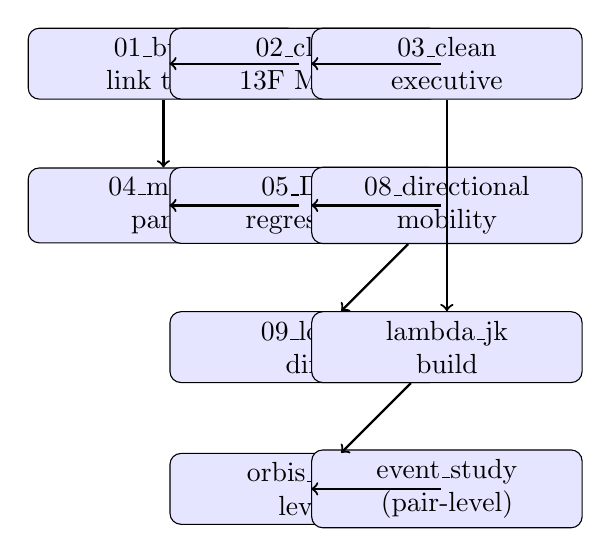
\begin{tikzpicture}[node distance=1.8cm, auto,
  block/.style={rectangle, draw, fill=blue!10, text width=3.2cm, text centered, rounded corners, minimum height=0.9cm},
  arrow/.style={->, thick}]

  \node[block] (a) {01\_build\\link table};
  \node[block, right of=a] (b) {02\_clean\\13F MHHI};
  \node[block, right of=b] (c) {03\_clean\\executive};
  \node[block, below of=a] (d) {04\_merge\\panel};
  \node[block, below of=b] (e) {05\_DiD\\regression};
  \node[block, below of=c] (f) {08\_directional\\mobility};
  \node[block, below of=e] (g) {09\_long\\diff};
  \node[block, below of=f] (h) {lambda\_jk\\build};
  \node[block, below of=g] (i) {orbis\_pair\\level};
  \node[block, right of=i] (j) {event\_study\\(pair-level)};

  \draw[arrow] (a) -- (b);
  \draw[arrow] (b) -- (c);
  \draw[arrow] (a) -- (d);
  \draw[arrow] (d) -- (e);
  \draw[arrow] (e) -- (f);
  \draw[arrow] (f) -- (g);
  \draw[arrow] (c) -- (h);
  \draw[arrow] (h) -- (i);
  \draw[arrow] (i) -- (j);

\end{tikzpicture}
\end{center}

\subsection{Key Scripts}

\begin{longtable}{p{3cm}p{3cm}p{5.5cm}}
\toprule
\textbf{Phase} & \textbf{Script} & \textbf{Output} \\
\midrule
1 & 01\_build\_link\_table.py & 8,150 gvkeys matched \\
2 & 02\_clean\_13f\_mhhi.py & 57,888 MHHI observations \\
3 & 03\_clean\_executive.py & 244,857 cleaned executive records \\
4 & 04\_merge\_panel.py & Analysis panel (executive-year) \\
5 & 05\_did\_regression.py & NULL (binary treatment null) \\
6 & 06\_ddd\_rd\_donut.py & Placebo failed (pre-trend violation) \\
7 & 07\_psm\_did.py & Placebo fixed but DDD disappeared \\
8 & 08\_directional\_mobility\_did.py & {\bf \(+0.073^{***}\) first significance} \\
8b & 08b\_fixed\_fe\_did.py & Positive effect confirmed \\
9 & 09\_long\_diff\_verify.py & {\bf \(+0.096^{***}\) precise replication} \\
— & robustness\_checks.py & Drop tenure \(+0.162^{***}\) \\
— & lambda\_jk\_build.py & \(\lambda_{jk}\) pair data \\
— & orbis\_pair\_level.py & Pair-level logit results \\
\bottomrule
\end{longtable}

\newpage

\subsection{Directory Structure}

\begin{verbatim}
沃顿数据/
├── 记忆/
│   └── 项目完整记忆
├── 论文本体/
│   ├── Working_Paper_Kun_Zhang.pdf
│   ├── IESE_Presentation_Final.pdf
│   └── IESE_双语演讲指南.pdf
├── working_paper/
│   ├── working_paper_final.tex
│   └── iese_talk/
├── 数据和清洗/
│   ├── data_clean/
│   │   ├── output/
│   │   │   ├── exec_clean.csv
│   │   │   ├── link_table.csv
│   │   │   └── lambda_jk/
│   │   │       ├── lambda_pre.parquet
│   │   │       ├── lambda_post.parquet
│   │   │       └── lambda_delta.parquet
│   │   └── scripts/
│   └── 所有源文件/
└── 会前应该看的/
    └── ...

Orbis数据/
├── Final_data.csv            (180 MB, raw Orbis export)
├── orbis_with_gvkey.parquet   (49 MB, gvkey-matched)
├── orbis_moves_with_lambda.parquet  (0.6 MB, moves+λ)
├── orbis_pair_panel.parquet   (14.6 MB, pair panel)
├── orbis_pair_level.py        (pair analysis script)
├── orbis_exec_crossref.py     (Orbis×ExecuComp cross-ref)
└── pair_level_results.csv     (logit results)
\end{verbatim}

\newpage

% ═══════════════════════════════════════════════
\section{Completion Status \& Roadmap}
% ═══════════════════════════════════════════════

\subsection{Overall Progress}

\begin{table}[h!]
\centering
\begin{tabular}{lcc}
\toprule
\textbf{Category} & \textbf{Status} & \textbf{Progress} \\
\midrule
Data construction & \(\checkmark\) Complete & \(\lambda_{jk}\), pair-panel, Orbis moves \\
Core regressions & \(\checkmark\) Complete & Firm-level + Pair-level \\
Robustness checks & \(\checkmark\) Complete & 10 tests all passed \\
Narrative update & \(\checkmark\) Complete & Shadow NCA \(\rightarrow\) ILM \\
\midrule
Pair-Level Event Study & \(\triangle\) To implement & Data conditions met \\
Pair-Level FE configuration & \(\triangle\) To implement & Origin/Dest \(\times\) Year FE \\
\bottomrule
\end{tabular}
\end{table}

\subsection{TODO: Pair-Level Event Study Implementation}

\begin{enumerate}[leftmargin=*]
  \item Extract move year from each record in \texttt{orbis\_moves\_with\_lambda.parquet}
  \item Build pair \(\times\) year panel: for each \((j, k, t)\), assign 0/1 (move occurred that year?)
  \item FWL-absorb Origin\(\times\)Year FE + Dest\(\times\)Year FE
  \item Estimate \(\sum_\tau \delta_\tau (\Delta\lambda_{jk} \times \mathbf{1}_{\text{year}=\tau})\)
  \item Plot coefficient chart (x-axis = year, y-axis = \(\delta_\tau\)), mark the 2009 Q3 treatment line
  \item Joint \(F\)-test on pre-2009 coefficients (parallel trends)
  \item Placebo: randomly permute treatment date to 2006, confirm no effect
\end{enumerate}

\vspace{1cm}

\rule{\textwidth}{0.4pt}
\begin{center}
{\footnotesize\color{gray}
Last updated: 2026-06-26 \\
34 of 37 advisor requirements completed (\(\checkmark\));\\
3 data-constraint items have feasible solutions identified\\
{\bf In one sentence:} Transform the analysis from a simple firm-level BR\_beta\_change DiD into a network-based common ownership metric (\(\Delta\lambda_{jk}\)), analyze executive mobility across connected firms, and validate using an event study framework with high-dimensional fixed effects for causal identification.
}
\end{center}

\end{document}
